\documentclass{article}

\textwidth=6.5in
\textheight=8.5in
\voffset=-54pt
\oddsidemargin=0in
\evensidemargin=0in
\setlength{\parskip}{8pt}
\setlength{\parindent}{0pt}

\usepackage{amsmath, amssymb}
\usepackage{ifthen}

\usepackage[inline]{enumitem}
\setlist{topsep=0pt, parsep=8pt}

\usepackage[rgb,table]{xcolor}\convertcolorsUfalse
\usepackage{graphicx}

% change hyperref options
\PassOptionsToPackage{hyphens}{url}
\usepackage[bookmarks,colorlinks,linkcolor=black,citecolor=blue,pdfstartview=FitH,urlcolor=blue]{hyperref}
\hypersetup{pdfpagemode=UseNone}
\usepackage{bookmark}

\usepackage{graphicx}
\usepackage{multicol}
\usepackage{framed}
\usepackage{array}

\usepackage{icomma}

\usepackage{soul}
\usepackage[normalem]{ulem}

\usepackage{pgfplots}
\pgfplotsset{compat=1.18}  
\pgfplotscreateplotcyclelist{mycolor}{black, blue, red, green!70!black, magenta, purple, cyan, orange }  
\pgfplotsset{
  disabledatascaling,
  cycle list=tikzcolor, 
  axis lines=middle,
  every axis plot/.style={no marks, thick},
  every axis/.style={
    enlarge x limits=false,
    enlarge y limits=auto,
    xlabel style={at={(current axis.right of origin)},anchor=west},
    ylabel style={at={(current axis.above origin)},anchor=south},
    % extra x and y ticks for asymptotes
    extra x tick style={grid=major, grid style={dashed,black}},
    extra y tick style={grid=major, grid style={dashed,black}},
    /pgf/number format/1000 sep={},
  },    
  tick label style = {font=\footnotesize, fill=\currentbgcolor, inner sep=0pt},    
  xticklabel shift=1pt,    
  scaled ticks=false,
  scaled y ticks=false,
  unbounded coords=jump,
  samples=101,
  minor tick length=0,
  scatter/classes={
    open={mark=*,draw=black,fill=white, mark size=2, thin},
    closed={mark=*,draw=black,fill=black, mark size=2, thin}
  },
  width=3in,
}
\pgfplotsset{open/.style={only marks, mark=*, fill=white, thin, mark size=2}}
\pgfplotsset{closed/.style={only marks, mark=*, draw=black, fill=black,
    thin, mark size=2}}
\pgfplotsset{labeled/.style={nodes near coords, only marks, mark=*, draw=black, fill=black, thin, mark size=2, point meta=explicit symbolic}}

\newcommand{\axes}[1][]{
  \begin{tikzpicture}
    \begin{axis}[xtick=\empty, ytick=\empty, ymin=-2, ymax=2,
      xmin=-4.25, xmax=4.25, #1]
    \end{axis}
  \end{tikzpicture}
}
\usepackage{tikz}
\usetikzlibrary{
  matrix,%
  % enables the snake paths
  decorations.pathmorphing,%
  % enables bigger arrows
  decorations.markings,%
  decorations.pathreplacing,%
  decorations.text,%
  calc,%
  patterns,%
  shapes.geometric,%
  arrows,
  decorations.shapes,
  positioning,
  plotmarks,
  intersections
}
\tikzset{>=latex} % sets default arrow type in tikz
\tikzset{font=\normalsize}
\tikzset{mark size=1.5pt, mark options=thin}
\tikzset{pin distance=4pt,
  every pin edge/.style={<-, thin, shorten <= -2pt}}

\interfootnotelinepenalty=10000
\renewcommand{\thefootnote}{(\arabic{footnote})}

\usepackage{multirow, bigdelim}

% change to \usepackage[sols]{handout} to see solutions
\usepackage[sols, notes]{handout}

\newcommand\iscurrentenumi[1]{%
  \ifthenelse{\equal{#1}{\theenumi}}{}{#1}}
\setenumerate[1]{ref=\#\arabic*}
\setenumerate[2]{ref=\protect\iscurrentenumi{\theenumi}(\alph*)}
\newcommand\enumiiprefix[2]{%
  \ifthenelse{{\equal{#1}{\theenumi}}\AND{\equal{#2}{(\alph{enumii})}}}{}{}%
  \ifthenelse{{\equal{#1}{\theenumi}}\AND{\NOT{\equal{#2}{(\alph{enumii})}}}}{#2}{}%
  \ifthenelse{\equal{#1}{\theenumi}}{}{#1#2}%
}
\setenumerate[3]{ref=\protect\enumiiprefix{\theenumi}{(\alph{enumii})}\roman*}

\newlength{\tipmargin}
\makeatletter

\renewenvironment{framed}{
  \setlength{\tipmargin}{\textwidth-\linewidth}
  \advance\@totalleftmargin-\tipmargin
  \def\FrameCommand{\hspace{\tipmargin}\fbox}%
  \advance\linewidth\tipmargin
  \MakeFramed {\advance\hsize-\width \FrameRestore}%
}
{\endMakeFramed}

\makeatother

\definecolor{purple}{rgb}{0.5,0,1.0}

\usepackage{fancyhdr}
\lhead{\textcolor{white}{This content is protected and may not be shared, uploaded, or distributed.}}
\rhead{}
\rfoot{\vspace*{\fill}\footnotesize\textcopyright{} \emph{Harvard Math Ma}}
\renewcommand{\headrulewidth}{0pt}
\pagestyle{fancy}
\begin{document}

\htitle{A Library of Basic Functions and Properties}

\begin{problemonly}
  \begin{framed}

You should be able to:
    \begin{itemize}[topsep=0pt,partopsep=0pt,parsep=8pt,itemsep=0pt]
    \item Sketch and recognize graphs of $y = mx + b$, $y = x^2$, $y = x^3$, $y = \frac{1}{x}$, $y = \frac{1}{x^2}$, $y = |x|$, and $y = \sqrt{x}$.

    \item Understand the following characteristics of a function graphically: positive / negative, increasing / decreasing, intercepts, asymptotes, continuity, concavity, even / odd.

    \item Algebraically determine whether a function is even, odd, or neither.

    \item Explain what it means to say a function is increasing / decreasing \emph{without bound}, as opposed to having an \emph{upper bound} or \emph{lower bound}.

    \item Recognize when the graph of a function given algebraically has a hole and construct algebraic examples of functions whose graphs have holes.

    \end{itemize}
  \end{framed}
\end{problemonly}

\begin{enumerate}
\item  \label{concavity-reminder}

  \note{I'll start class by having students try this quickly.}

  \begin{problem}[1.5in]
    \emph{Warm up.} Last time, we talked about what it meant graphically for a function to be \uline{concave up} or \uline{concave down}. Write down / sketch what these terms mean. Can a function be neither?
  \end{problem}

  \begin{solution}
    The graph of a \emph{concave up} function curves ``up like a cup.''
    The graph of a \emph{concave down} function curves ``down like a frown.''
    A linear function is neither concave up nor concave down.
  
    \begin{center}
    \begin{tabular}{c c c c c}
      \begin{tikzpicture}
          \begin{axis}[width=1.75in, xtick=\empty, ytick=\empty]
            \addplot+[domain=1:3]{(x-2)^2+2};
        \end{axis}
      \end{tikzpicture} &&
      \begin{tikzpicture}
          \begin{axis}[width=1.75in, xtick=\empty, ytick=\empty]
            \addplot+[domain=1:3]{-(x-2)^2+4};
        \end{axis}
      \end{tikzpicture} &&
      \begin{tikzpicture}
          \begin{axis}[width=1.75in, xtick=\empty, ytick=\empty]
            \addplot+[domain=1:3]{x+1};
        \end{axis}
      \end{tikzpicture} \\
      concave up && concave down && linear
    \end{tabular}
    \end{center}
  \end{solution}

  \note{Then, I'll give a bit of an intro to what we're doing today, along the lines of: Last class, we looked at functions described verbally and graphically. We often want to come up with algebraic formulas for functions so that we can get quantitative information about them. We do this by building a library of functions we're familiar with; when we want to model something, we can see if something in our library is a useful starting point.}

\item  \label{basic-graphs-2-sketch}

  \note{I'll have students try this on their own for a couple of minutes, just so that I can get a sense of which students will need more support. I won't give students much time for this because my main goal is just to emphasize that:
    \begin{itemize}[nosep]
    \item A useful strategy is to plug in points / make a table.
    \item These graphs are worth memorizing because we'll use them so much. 
    \end{itemize}
    When we discuss, I will try to spend a little time on how these graphs relate to each other. For example, they all intersect at $(1, 1)$; on $(1, \infty)$, $x < x^2 < x^3$, but on $(0, 1)$, the order is reversed.}

  \begin{problem}
    On the axes below, sketch graphs of $f(x) = 1$, $g(x) = x$, $h(x) = x^2$, and $j(x) = x^3$ (and label which is which).
  \end{problem}

  \begin{problemonly}
    \axes[xmin=-4.25, xmax=4.25, ymin=-4.25, ymax=4.25, axis equal
    image, width=3.5in, xtick={-4, -3, ..., 4}, ytick={-4, -3, ..., 
      4}] 
  \end{problemonly}

  \begin{solution}
    We'll use these four functions very frequently, so you should take time to
    memorize their graphs. You can build stronger memories by quizzing yourself on
    questions like ``Why does the graph look like this?'' Another important fact
    to remember is that
    $1 < x < x^2 < x^3$ on the interval $(1,\infty)$, but
    $x^3 < x^2 < x < 1$ on $(0,1)$.

    \pgfplotsset{style a/.style={domain=-4.25:4.25,
    restrict y to domain=-4.25:4.25}}
    \begin{tikzpicture}
      \begin{axis}[xmin=-4.25, xmax=4.25, ymin=-4.25, ymax=4.25,
                   axis equal image, width=3.5in, 
                   xtick={-4, -3, ..., 4}, ytick={-4, -3, ..., 4},
                   clip = false
      ]
      
        \addplot[style a, purple]{1};
        \node at (4,0.6) {\textcolor{purple}{$f$}};
        
        \addplot[style a, orange]{x};
        \node at (4,3.6) {\textcolor{orange}{$g$}};

        \addplot[style a, red]{x^2};
        \node at (2.4,4) {\textcolor{red}{$h$}};
        
        \addplot[style a, black, samples=400]{x^5};
        \node at (1.1,4) {$j$};
        
      \end{axis}
    \end{tikzpicture}

  \end{solution}

\item  \label{basic-graphs-2-characterization}

  \emph{Characterizing functions.}
  \begin{enumerate}
  \item

    \note{Be sure to explain the notation $(-\infty, \infty)$.

      Only $f(x) = 1$ is positive on $(-\infty, \infty)$, but I'll point out $h(x) = x^2$ is positive everywhere except 0. We could say it's non-negative on $(-\infty, \infty)$.}

    \begin{problem}[\vfill]
      Which of the functions in \ref{basic-graphs-2-sketch} are \textbf{positive} on $(-\infty, \infty)$?
    \end{problem}

    \begin{solution}
      Only $f$ is positive on $(-\infty,\infty)$. Since $h(0)=0$,
      we can't say that $h$ is positive on $(-\infty, \infty)$.  
      We can say that $h$ is positive on $(-\infty, 0) \cup (0, \infty)$, 
      or we can say that $h$ is \uline{non-negative} on $(-\infty, \infty)$.
      Both $g$ and $j$ are negative on $(-\infty, 0)$ and positive on $(0, \infty)$.
    \end{solution}

  \item
    \begin{problem}[\vfill]
      Which of the functions in \ref{basic-graphs-2-sketch} are \textbf{increasing} on $(-\infty, \infty)$?
    \end{problem}

    \begin{solution}
      Only $g$ and $j$ are increasing on $(-\infty, \infty)$. Since $f$ is a constant function,
      it is neither increasing nor decreasing. 
      The function $h$ is decreasing on $(-\infty,0)$ and
      increasing on $(0,\infty)$.
      \footnote{Our textbook would say that $h$ is decreasing on $(-\infty, 0]$
      and increasing on $[0, \infty)$. In Math Ma, we aren't going to be picky about whether you
      include the endpoints when describing where a function is increasing or decreasing. 
      If you're curious about this, come ask about it in office hours!}
    \end{solution}

  \item
    \begin{problem}[\vfill]
      Which of the functions in \ref{basic-graphs-2-sketch} are \textbf{linear} on $(-\infty, \infty)$?
    \end{problem}

    \begin{solution}
      Only $f$ and $g$ are linear on $(-\infty, \infty)$. For either function, the graph is a straight 
      line with a certain slope, meaning that the function has a constant rate of change.
    \end{solution}

  \item 
    \begin{problem}[\vfill]
      Which of the functions in \ref{basic-graphs-2-sketch} are \textbf{concave up} on $(-\infty, \infty)$?
    \end{problem}

    \begin{solution}
      Only $h$ is concave up on $(-\infty, \infty)$. Both $f$ and $g$ are neither concave up nor concave down on $(-\infty, \infty)$. The function $j$ is concave down
      on $(-\infty,0)$ and concave up on $(0,\infty)$.
    \end{solution}
  \end{enumerate}

  \begin{framed}
    \emph{Two types of symmetry.} We say that a function is \uline{even} if its graph is symmetric over the vertical axis and \uline{odd} if, when you rotate it $180^\circ$ about the origin, the result is the same as the original. Here are a few examples:
    \begin{center}
      \begin{tabular}{c c c c c c c}
        \begin{tikzpicture}
          \begin{axis}[xtick=\empty, ytick=\empty, width=1.6in]
            \addplot+[domain=-1.2:1.2]{x^2 * (x^2 - 1) - 0.1};
          \end{axis}
        \end{tikzpicture} &&
        \begin{tikzpicture}
          \begin{axis}[xtick=\empty, ytick=\empty, width=1.6in, 
            ymin=0] 
            \addplot+[sharp plot] coordinates { (-2, 1) (-1.5, 3)
              (-0.5, 3)}; % 
            \addplot+[sharp plot] coordinates { (2, 1) (1.5, 3)
              (0.5, 3)}; %
            \addplot+[closed] coordinates { (-0.5, 3) (0.5, 3)
            }; % 
          \end{axis}
        \end{tikzpicture} &&
        \begin{tikzpicture}
          \begin{axis}[xtick=\empty, ytick=\empty, width=1.6in]
            \addplot+[domain=-pi:pi, samples=201]{2*sin(deg(x)) + (2*sin(deg(3*x)))/3 + (2*sin(deg(5*x)))/5 + (2*sin(deg(7*x)))/7 + (2*sin(deg(9*x)))/9 + (2*sin(deg(11*x)))/11};
          \end{axis}
        \end{tikzpicture} &&
        \begin{tikzpicture}
          \begin{axis}[xtick=\empty, ytick=\empty, width=1.6in]
            \addplot+[domain=-4:-1]{-atan(x)};
            \addplot+[domain=1:4]{-atan(x)};
            \addplot+[closed] coordinates {(-1, 45) (1, -45)};
          \end{axis}
        \end{tikzpicture} \\
        even && even && odd && odd
      \end{tabular}
    \end{center}
  \end{framed}

  \begin{enumerate}[resume]
  \item 

    \begin{problem}[\vfill]
      Which of the functions in
      \ref{basic-graphs-2-sketch} are \textbf{even}?  
    \end{problem}

   \begin{solution}
      Only $f$ and $h$ are even. Both of their graphs are symmetric about the $y$-axis.
   \end{solution} 

    \begin{problem}[\vfill]
      Which are \textbf{odd}?
    \end{problem}

    \begin{solution}
      Only $g$ and $j$ are odd. Both of their graphs are symmetric about the origin.
    \end{solution}
  \end{enumerate}

\end{enumerate}
\begin{framed}
  Come up with algebraic definitions of even and odd:

  \begin{itemize}
  \item A function $f(x)$ is \uline{even} if \fitb{3.5in}{$f(-x) = f(x)$ for all $x$ in the domain of $f$}.
  \item A function $f(x)$ is \uline{odd} if \fitb{3.5in}{$f(-x) = -f(x)$ for all $x$ in the domain of $f$}.
  \end{itemize}

  \emph{One more important property!} The functions in \ref{basic-graphs-2-sketch} are all \emph{continuous} on $(-\infty, \infty)$, meaning that we can sketch each graph without picking up our pencil.
\end{framed}

\pspace{\newpage}

\begin{enumerate}[resume]
\item  \label{graph-with-pinhole-1} Let $\displaystyle f(x) = \frac{x^2 (x - 1)}{x - 1}$.

  \begin{enumerate}
  \item \label{graph-with-pinhole-1-domain}

    \note{It's worth helping students understand why $\frac{0}{0}$ is undefined. I like to do this by having students remember why $\frac{6}{2} = 3$; it's just another way of saying $6 = 2 \cdot 3$. Then, writing $\frac{0}{0} = a$ is the same as $0 = 0 \cdot a$, but this is true for every real number $a$, so there isn't a single value that we can define $\frac{0}{0}$ to be.}

    \begin{problem}[0.25in]
      What's the domain of $f$?
    \end{problem}

    \begin{solution}
        For all values of $x$ except $x=1$, the output $f(x)$ is a defined number. 
        When $x=1$, the expression
        $f(1)=\dfrac{(1)^2(1-1)}{1-1}$ involves division by zero, which is undefined. Therefore the
        domain of $f$ is $(-\infty, 1) \cup (1, \infty)$.
    \end{solution}
  \item

    \note{Be sure to explain the ``empty hole'' convention for representing a hole in a graph. It's also worth talking about how tiny this hole really is.}

    \begin{problem}[2in]
      Sketch the graph of $f$. Make sure your answer is consistent with your answer to \ref{graph-with-pinhole-1-domain}.
    \end{problem}

    \begin{solution}

      \begin{tikzpicture}
          \begin{axis}[xmin=-2.25, xmax=2.25, xtick distance=1,
                       ymin=-0.25, ymax=4.25, ytick distance=1,
                       width=2.25in,
          ]
            \addplot[domain=-2.25:2.25]{x^2};
            \addplot[open] coordinates {(1,1)};
          \end{axis}
      \end{tikzpicture}
        
      If $x \neq 1$, then we can cancel $x-1$ in the numerator and denominator and determine that
      for all values of $x$ \uline{except $x=1$}, $f(x)=x^2$. This means that the graph of $f$ looks
      almost identical to the graph of $y=x^2$. However, 
      since $f(1)$ is undefined, the graph should have a ``hole'' at the corresponding
      point on the graph of $y=x^2$, which is $(1,1)$.

    \end{solution}
    
  \item

    \note{This is our first example of a discontinuous function, so I will introduce the terminology ``discontinuous at $1$''.}

    \begin{problem}[0.5in]
      Is $f$ continuous on $(-\infty, \infty)$? 
    \end{problem}

    \begin{solution}
      No. Our working definition is that a function is continuous on an interval
      if we can draw its graph without lifting our pencil off of the paper.
      We would have to lift our pencil off of the paper because of the hole.
      We say that the function is \uline{discontinuous at $1$}. 
    \end{solution}
  \end{enumerate}

\item  \label{basic-graphs-1-think-of-function}

  In each part, think of a function $f(x) = \fitb{0.5in}{}$ whose graph
  looks like the given picture. Also, fill in the blanks / answer the
  other questions in each part.

  \begin{enumerate}
  \item

    \note{The question about intercepts is just to make sure students are familiar with this language.}

    \begin{minipage}[t]{2.1in}
      \vspace{0pt}
      \raisebox{2ex-\height}{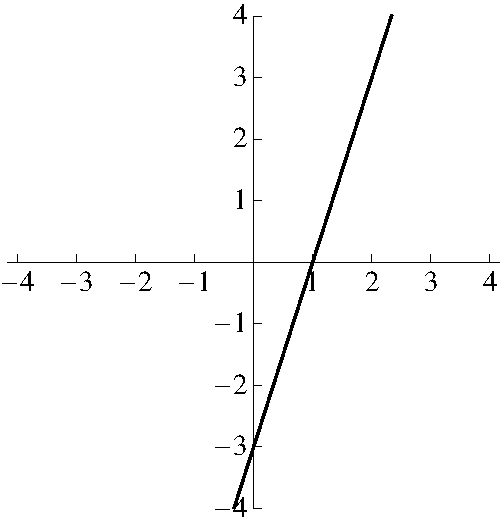
\includegraphics[width=2in]{images/basic-graphs-1-1}}
    \end{minipage}
    \hspace{0.25in}
    \begin{minipage}[t]{\linewidth-2.45in}
      \setlength{\parskip}{8pt}
      \begin{itemize}
      \item $f(x) = \fitb{1in}{3x - 3}$

      \item 
        $f$ has $x$-intercept(s) $\fitb{1in}{1}$

        $f$ has $y$-intercept $\fitb{1in}{-3}$
      \end{itemize}

    \end{minipage}

    \pspace{0.25in}

    \note{It's easy for students to think every function must be even or odd, so this is our first counterexample to that idea. I will also have them calculate $f(-x)$ and $- f(x)$ just to make sure they're clear on the difference between them.}

    \begin{problem}[\vfill\newpage]
      Is $f$ even? Is $f$ odd? Explain both geometrically and
      algebraically.
    \end{problem}

    \begin{solution}
        The function $f$ is neither even nor odd. Geometrically, this is because the graph is
        neither symmetric about the $y$-axis nor symmetric about the origin. Algebraically, this
        is because $f(-x)=-3x-3$ is neither equal to $f(x)=3x-3$ nor $-f(x)=-3x+3$.
    \end{solution}

  \item \label{library-|x|}

    \note{I've asked where this is positive just so we can discuss the union notation $(-\infty, 0) \cup (0, \infty)$.

      Robin's book uses the convention that this is decreasing on $(-\infty, 0]$ and increasing on $[0, \infty)$. We're not going to be picky about whether they include endpoints when they say where a function is increasing or decreasing; I'm guessing students might find it more natural to say the function is decreasing on $(-\infty, 0)$ and increasing on $(0, \infty)$, and that's totally fine.}

    \begin{minipage}[t]{2.1in}
      \vspace{0pt}
      \raisebox{2ex-\height}{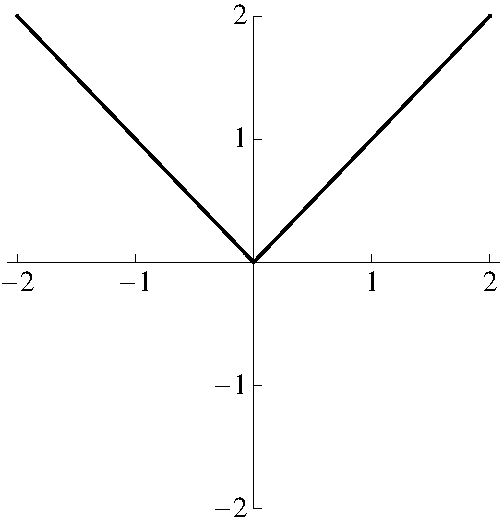
\includegraphics[width=2in]{images/basic-graphs-1-3}}
    \end{minipage}
    \hspace{0.25in}
    \begin{minipage}[t]{\linewidth-2.45in}
      \begin{itemize}
      \item $f(x) = \fitb{1in}{|x|}$

      \item 
        $f$ is positive on $\fitb{1.5in}{(-\infty, 0) \cup (0, \infty)}$

        $f$ is negative on \fitb{1.5in}{nowhere}

      \item $f$ is increasing on
        $\fitb{1.5in}{(0,\infty)}$

        $f$ is decreasing on $\fitb{1.5in}{(-\infty,0)}$

      \end{itemize}
    \end{minipage}      

    \note{This is to remind me to talk about the piecewise formula.}

    \begin{problem}[1in]
      We can see that the graph is made up of two pieces of lines. (So, we say $f$ is \emph{piecewise linear}.) What are the equations for those lines?
    \end{problem}

    \begin{solution}
      The right piece is part of $y = x$, and the left piece is part
      of $y = -x$. So, we can also write a piecewise formula for $f$:
      \[ f(x) =
        \begin{cases}
          x & \text{ when } x \geq 0 \\
          -x & \text{ when } x < 0 \\
        \end{cases}\]
    \end{solution}

  \end{enumerate}

\item  \label{basic-graphs-1-sketch}

  \note{It's helpful to first see whether a function is even or odd because, if it is, we can just focus on sketching the right half of the graph and then use symmetry to fill in the left half. For the right half, making a table of values can help; you can also encourage students to think qualitatively (``If $x$ is positive and increasing, then $\frac{1}{x}$ decreases and gets close to 0'').

    I haven't asked about asymptotes because students might not know the word, but I will introduce them here.

    I don't plan to go over the answer to every single question here for all 3 functions. }

  For each of the following functions:
  \begin{itemize}[itemsep=0pt, parsep=0pt]
  \item What is the domain?
  \item Use the algebraic definitions of even and odd to determine whether the function is even, odd, or neither.
  \item Sketch the graph of the function. 
  \item Where is the function concave up?  Where is it concave down?
  \end{itemize}

  \probonly{\begin{multicols}{3}}
    \begin{enumerate}
    \item

      \begin{problem}[2.25in]
        $\displaystyle f(x) = \frac{1}{x}$
      \end{problem}

      \begin{solution}
        \
        
        \raisebox{2ex-\height}{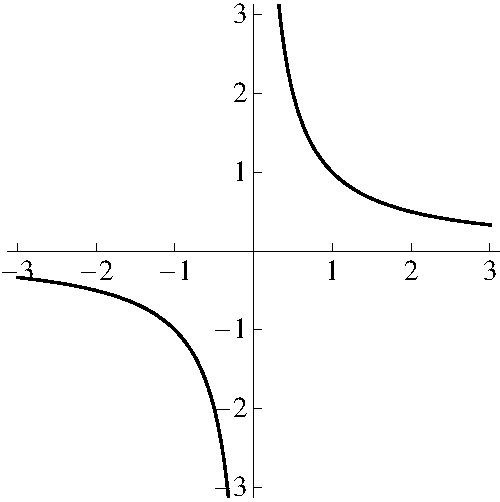
\includegraphics[width=2.25in]{images/basic-graphs-1-5}}

        \begin{itemize}

        \item The domain is all non-zero numbers, which we write in
          interval notation as $(-\infty, 0) \cup (0, \infty)$, and
          the range is also $(-\infty, 0) \cup (0, \infty)$.

        \item Since $f(-x) = \dfrac{1}{-x}$ and $- f(x) = -
          \dfrac{1}{x}$, we see that $f(-x) = - f(x)$, so $f$ is odd.

        \item $f$ is decreasing on $(-\infty, 0) \cup (0, \infty)$.

        \item $f$ is concave up on $(0, \infty)$ and concave down on
          $(-\infty, 0)$.

        \item To graph this function, we have to pick up our pencil or
          chalk; it's not all in one piece.  In particular, we have to
          pick up our pencil at $x = 0$, so we say that the function is
          \uline{discontinuous at 0}.

          This discontinuity has a particular name; it's called a
          \uline{vertical asymptote}. What this means is that, as $x$
          gets close to 0, the size of $f(x)$ increases without bound.
          Visually, the graph gets closer and closer to the vertical
          line $x = 0$ without touching it.

          This graph also has a \uline{horizontal asymptote}. A
          horizontal asymptote is a horizontal line that the graph
          approaches as $x$ gets very big or $x$ gets very negative.
        \end{itemize}
      \end{solution}

    \item

      \begin{problem}[2.25in]
        $\displaystyle f(x) = \frac{1}{x^2}$
      \end{problem}

      \begin{solution}
        \
        
        \raisebox{2ex-\height}{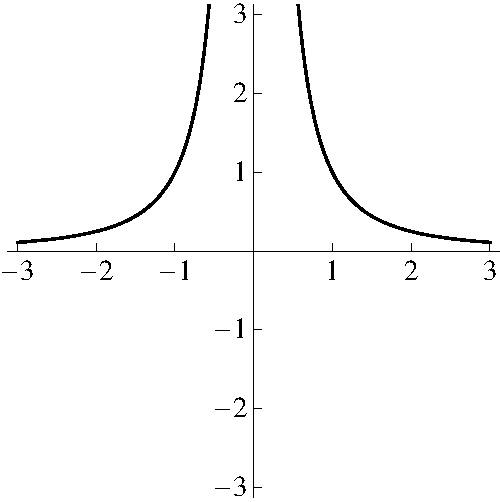
\includegraphics[width=2.25in]{images/basic-graphs-1-7}}        

        \begin{itemize}
        
          \item The domain is $(-\infty, 0) \cup (0, \infty)$. The range is $(0, \infty)$.

          \item Since $f(-x)=\dfrac{1}{(-x)^2}=\dfrac{1}{x^2}$, we see that $f(-x)=f(x)$,
          so $f$ is even.

          \item $f$ is increasing on $(-\infty, 0)$ and decreasing on $(0, \infty)$.

          \item $f$ is concave up on $(-\infty, 0) \cup (0, \infty)$. 

          \item The function is discontinuous at $0$. It has a vertical asymptote, $x=0$, and
          a horizontal asymptote, $y=0$. 
          
        \end{itemize}
      \end{solution}

    \item

      \note{I will talk about the domain here since the endpoint is included, and I want to make sure they see the square bracket notation for that.}

      \begin{problem}[2.25in]
        $f(x) = \sqrt{x}$
    \end{problem}

    \begin{solution}
      \

      \raisebox{2ex-\height}{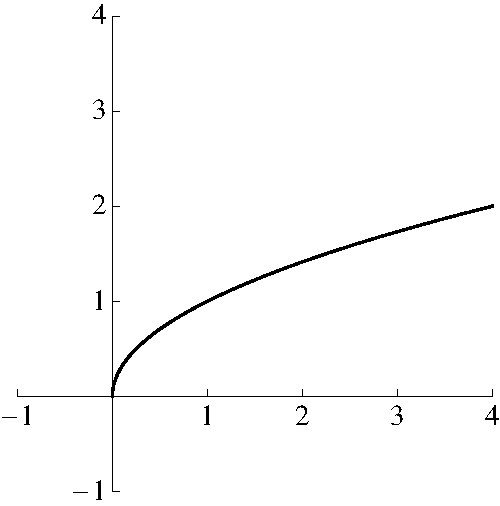
\includegraphics[width=2.25in]{images/basic-graphs-1-8}}
      
        \begin{itemize}
        
          \item The domain is $[0, \infty)$. The range is also $[0, \infty)$.

          \item Since the domain of $f$ includes only non-negative numbers, $f(-x)$ is
          undefined except when $x=0$, meaning $f$ is neither even nor odd. This is consistent with
          the graph, which is neither symmetric about the $y$-axis nor about the origin.

          \item $f$ is increasing on $[0,\infty)$.

          \item $f$ is concave down on $[0,\infty)$.

          \item $f$ continuous on $[0,\infty)$. 
          
        \end{itemize}
    \end{solution}

    \end{enumerate}
    \probonly{\end{multicols}}

  \pspace{\newpage}

\item  \label{bounded-vs-without-bound}
  \begin{enumerate}

  \item

    \note{I will try to remember to contrast this with the left piece of $\frac{1}{x}$, which decreases without bound.}

    \begin{problem}[0.75in]
      Two of the functions in \ref{basic-graphs-1-sketch} are decreasing on $(0, \infty)$. Do they have a \textbf{lower bound} (a value that they never get below) on $(0, \infty)$, or do they \textbf{decrease without bound} on $(0, \infty)$?
    \end{problem}

    \begin{solution}
      Both $\frac{1}{x}$ and $\frac{1}{x^2}$ are decreasing on $(0,\infty)$. On this interval,
    both have a lower bound of $0$. As $x$ takes on ever higher positive values, 
      both functions output ever lower positive numbers, never going below 0.
    \end{solution}

  \item
    \begin{problem}[0.5in]
      The other function in \ref{basic-graphs-1-sketch} is increasing on $(0, \infty)$. Does it have an \textbf{upper bound} (a value that it never gets above) on $(0, \infty)$, or does it \textbf{increase without bound} on $(0, \infty)$?
    \end{problem}

    \begin{solution}
      The function $\sqrt{x}$ increases on $[0,\infty)$. As $x$ takes on ever higher positive
      values, the function outputs ever higher positive numbers, therefore the function increases
      without bound.
    \end{solution}

  \end{enumerate}

\item  \label{horizontal-asymptote-misconceptions}

  \note{This is intentionally an example where the graph crosses its horizontal asymptotes. However, it isn't important to address this today.}

  \emph{A more interesting example of horizontal asymptotes.}

  \begin{problem}
    Here's the graph of a function $f(x)$ that has \emph{two}
    horizontal asymptotes. What are they (roughly)?

    \begin{tikzpicture}
      \begin{axis}[ytick={-3, -2, ..., 3}, xtick=\empty, width=4in, height=2in]
        \addplot+[domain=-20:-2] { atan(x) / 45 + 5 * x *
          e^(-x^2) }; %
        \addplot+[domain=-2:2] { atan(x) / 45 + 5 * x *
          e^(-x^2) }; %
        \addplot+[domain=2:20] { atan(x) / 45 + 5 * x *
          e^(-x^2) }; %
        \begin{solonly}
            \addplot[domain=-20:20, dotted, red]{-2};
            \addplot[domain=-20:20, dotted, red]{2};
        \end{solonly}
      \end{axis}
    \end{tikzpicture}
  \end{problem}

  \begin{solution}
    The function has \fbox{$y=2$} and \fbox{$y=-2$} as horizontal asymptotes. 
    As $x$ takes on lower and lower
    negative values, the output $f(x)$ eventually approaches $-2$. 
    As $x$ takes on higher and higher positive values, the output $f(x)$ eventually approaches $2$. 
    Note that the graph of a function can cross a horizontal asymptote! 
  \end{solution}
\item 

  \note{This is just more practice with piecewise formulas, as well as a chance to talk about how we sketch what's happening at 3 (the empty circle / filled circle convention). Again, it's okay if you don't get here; we'll have opportunities later to talk about this.}

  \begin{problem}[\vfill]
    Sketch the graph of the function
    \[ f(x) =
      \begin{cases}
        1 & \text{ if } x < 3 \\
        x & \text{ if } x \geq 3
      \end{cases}
    \] 
  \end{problem}

  \begin{solution}

    \begin{tikzpicture}
      \begin{axis}[xmin=-0.25, xmax=5.25, xtick distance=1,
                   ymin=-0.25, ymax=5.25, ytick distance =1,
                   width=2.5in, 
      ]

        \addplot[domain=-0.25:3]{1};
        \addplot[open] coordinates {(3,1)};
        \addplot[domain=3:5.25]{x};
        \addplot[closed] coordinates {(3,3)};
      \end{axis}
    \end{tikzpicture}
    
    The function is defined in two pieces. On the interval $(-\infty,3)$, the graph of the function
    looks like the graph of $y=1$. On the interval $[3,\infty)$, the graph of the function looks like
    the graph of $y=x$. To show that $f(3)$ is $3$ and not $1$, we draw a filled circle at
    $(3,3)$ and an empty circle at $(1,3)$. 

    
  \end{solution}

\item 

  \note{This is a really common first instinct for students, even though \ref{graph-with-pinhole-1} should have showed them that this idea is wrong.}

  \begin{problem}[\nstretch{0.5}]
    True or false: If a function has a formula that looks like $f(x) = \dfrac{\text{something}}{x}$, then $f$ must have a vertical asymptote at $x = 0$.
  \end{problem}

  \begin{solution}
    False! A counterexample (that is, an example showing this is false) is $f(x) = \dfrac{x}{x}$. What does the graph of this look like?
  \end{solution}

\item  \label{even-odd-1}

  Algebraically determine whether each of the following is even, odd, or neither.
  \begin{enumerate}
  \item
    \begin{problem}[\vfill]
      $f(x) = -3x^4 + 6x^2 + 1$
    \end{problem}

    \begin{solution}
      We want to see how $f(-x)$ relates to $f(x)$.  Let's simplify
      $f(-x)$:
      \begin{align*}
        f(-x) &= -3 (-x)^4 + 6 (-x)^2 + 1\\
        &= -3 x^4 + 6x^2 + 1 
      \end{align*}
      This is the same as $f(x)$, so $f(x)$ is \fbox{even}.
    \end{solution}

  \item
    \begin{problem}[\stretch{2}]
      $\displaystyle g(x) = x^3 + {x^2} + 1$
    \end{problem}

    \begin{solution}
      We want to see how $g(-x)$ relates to $g(x)$.
      \begin{align*}
        g(-x) &= (-x)^3 + {(-x)^2} + 1 \\
        &= -x^3 + x^2 + 1
      \end{align*}
      This is not the same as $g(x)$, so the function is not even.
      This is also not the same as $-g(x)$, so the function is not
      odd. Therefore, $g(x)$ is \fbox{neither even nor odd}.
    \end{solution}
  \end{enumerate}

\end{enumerate}
\end{document}
